\documentclass[a4paper]{article}

\usepackage[spanish, es-tabla, es-nodecimaldot]{babel}
\usepackage[T1]{fontenc}
\usepackage[utf8]{inputenc}
\usepackage{lmodern}
\usepackage{amsmath, amssymb}
\usepackage{stackengine}
\usepackage{graphicx}
\usepackage[hmargin=1.8cm, vmargin=2cm]{geometry}
\usepackage[separate-uncertainty=true, per-mode=symbol]{siunitx}
\usepackage[small]{titlesec}
\usepackage[bottom]{footmisc}
\usepackage{float}
\usepackage{enumitem}
\usepackage{tikz}
\usepackage[font=small, labelfont=bf, labelsep=period]{caption}
\usepackage{subcaption}
\usepackage[colorlinks=true]{hyperref}

\newcommand{\letrita}[1]{\textsf{\textbf{\footnotesize{(#1)}}}} 

\title{\large{\textbf{Caracterización del generador de número aleatorios del Kilobot o \emph{Moneda}}}}
\author{%
	\normalsize{Tomás Ayala y Romina D'Alessandro}
}
\date{}

\begin{document}
	
\maketitle

Corrimos \href{https://github.com/rldromina/Kilobots/blob/tom/Moneda/moneda.c}{\texttt{moneda.c}}, usando siempre la función \texttt{rand\_hard()}.
Dejamos fijo el tiempo mínimo de prendido/apagado del LED del Kilobot a \texttt{TIME = 1000} (milisegundos).
Registramos varias filmaciones de 15 minutos del Kilobot ``tirando la moneda'' y una de 1 hora.

De cada medición obtenemos un \texttt{.csv} que en sus columnas tiene (i) la intensidad (en un entorno) del LED, con valores entre 0 y 255, y (ii) el instante del tiempo correspondiente. Graficamos la evolución temporal $I(t)$, su autocorrelación (ver la función \texttt{autocorrelación} de \href{https://github.com/rldromina/Kilobots/blob/tom/Moneda/aux.py}{\texttt{aux.py}}) y la frecuencia con las que ocurren las consecutividades\footnote{¿Existe esta palabra?} de longitud $n$. Por ejemplo, si la moneda en una tirada arrojó HTHTTTHHTHHHHHH, la consecutividad de longitud $n=1$ se presentó $4$ veces (H,T,H,T); la de $n=2$, $1$ vez (HH); la de $n=3$, 1 vez (TTT); la de $n=4$ y $n=5$, ninguna y $n=6$, 1 vez (HHHHHH). Notar que consecutividades de cara o ceca contribuyen por igual.

\begin{figure}[!h]
	\centering
	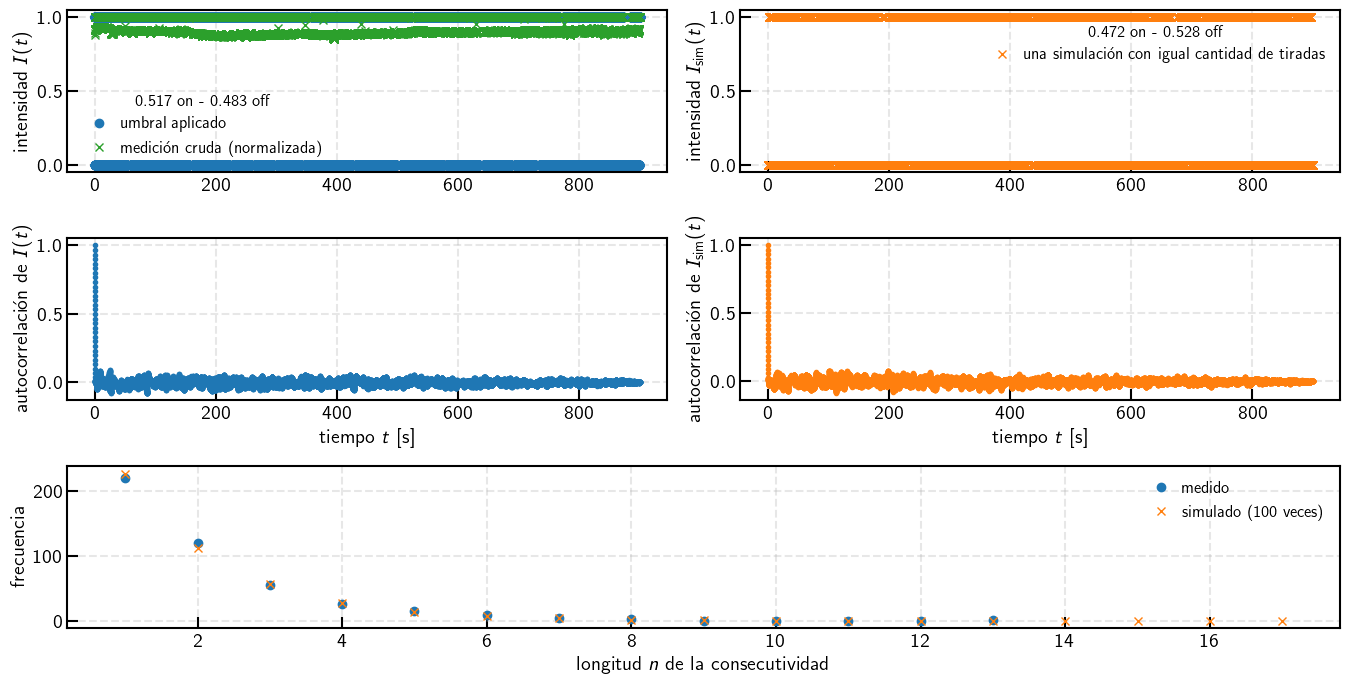
\includegraphics[width=\linewidth]{Resultados/15min_b.png}
	\caption{15 minutos.}
\end{figure}

La medición cruda fue tomada, parece, con mucha luz ambiental. Por eso cuando el LED estaba apagado, el valor de la intensidad está más cerca de saturar\footnote{Los valores presentados en verde están normalizados, o sea, divididos por 255.} (255) que de cero. Aun así se logra distinguir los dos estados del Kilobot. Para el análisis le pasamos un \href{https://github.com/rldromina/Kilobots/blob/tom/Moneda/aux.py}{umbral} que asigna sólo dos valores: 1 (prendido) y 0 (apagado).

En naranja se presenta el resultado de una simulación de la moneda tirada $900$ veces ya que $\SI{15}{\minute} = \SI{900}{\second}$ y era \texttt{TIME = 1000}.

Las autocorrelaciones, en ambos casos medido y simulado, caen a cero en $\SI{1}{\second}$ o, equivalentemente, luego de $30$ puntitos.\footnote{Grabamos a $30$ fps y los frames los capturamos con una tasa $t = 1$, o sea, guardábamos $1$ de cada $t$ frames, quedándonos en este caso con todos los frames.}.

En Labo 7 notábamos que ocurrían consecutividades en las tiradas de longitud $n=12$ por ejemplo. Esto nos volvía locos, por eso es parte de la caracterización medir la frecuencia con las que estas consecutividades aparecen. También lo fue el cálculo de la autocorrelación: pensábamos que con altas consecutividades presentes, el tiempo de correlación iba a ser mayor al de una moneda ``ideal'' (i.e. simulada en python), pero no.



Nos focalizamos entonces en el conteo de consecutividades. Para esta medición, comparamos esta frecuencia de aparición de consecutividades con las de una moneda simulada. Presentamos, en naranja, la media de $100$ realizaciones, cada una con la misma cantidad de tiradas\footnote{Si la cantidad de tiradas es muuuy grande es posible, aunque poco probable, que aparezca una consecutividad de, por ejemplo, longitud $n=20$, lo cual es casi imposible si la cantidad de tiradas es $20$ e imposible si es menor.}. Me sorprendió mucho que las frecuencias medidas y simuladas concuerden tan bien. 

Resumiendo, lo medido (y de lo que sospechábamos) y lo simulado presenta el mismo comportamientos:
\begin{itemize}
	\item 51.7\% on - 48.3\% off vs. 47.2\% on - 52.8\% off
	\item tiempo de correlación $= \SI{1}{\second}$
	\item misma distribución de consecutividades (!)
\end{itemize}































\end{document}